\documentclass[a4paper,12pt]{article}
\usepackage{amsmath}
\usepackage{amsfonts}
\usepackage{amssymb}
\usepackage{geometry}
\usepackage{graphicx}
\usepackage[T1]{fontenc}  % Kodowanie czcionki z polskimi znakami
\usepackage[utf8]{inputenc}  % Kodowanie znaków UTF-8
\usepackage{polski}  % Obsługa polskich znaków
\geometry{margin=1in}

\title{Raport z ćwiczenia NUM3}
\author{Bartosz Satoła}
\date{23 listopada 2024}

\begin{document}

\maketitle

\section{Opis ćwiczenia}

Celem zadania jest wyznaczenie wektora $y$ będącego rozwiązaniem układu równań $y = A^{-1}x$, gdzie macierz $A$ jest macierzą czterodiagonalną o rozmiarze $N \times N$ o specjalnej strukturze. Elementy macierzy $A$ definiują następujące przekątne:
\begin{itemize}
    \item dolna przekątna zawiera wartości $0.3$,
    \item główna przekątna zawiera wartości $1.01$,
    \item przekątna nad główną zawiera wartości $\frac{0.2}{i}$ dla $i = 1, 2, \dots, N-1$,
    \item druga przekątna nad główną zawiera wartości $\frac{0.15}{i^3}$ dla $i = 1, 2, \dots, N-2$.
\end{itemize}

Wektor prawej strony $x$ jest wektorem o wartościach $x = (1, 2, \dots, N)^T$.

Macierz $A$ w postaci pełnej przyjmuje kształt:
\[
A =
\begin{pmatrix}
1.01 & \frac{0.2}{1} & \frac{0.15}{1^3} & 0 & \cdots & 0 \\
0.3 & 1.01 & \frac{0.2}{2} & \frac{0.15}{2^3} & \cdots & 0 \\
0 & 0.3 & 1.01 & \frac{0.2}{3} & \cdots & 0 \\
0 & 0 & 0.3 & 1.01 & \cdots & 0 \\
\vdots & \vdots & \vdots & \vdots & \ddots & \frac{0.15}{(N-2)^3} \\
0 & 0 & 0 & 0.3 & 1.01 & \frac{0.2}{N-1} \\
0 & 0 & 0 & 0 & 0.3 & 1.01 \\
\end{pmatrix}
\]

Należy wyznaczyć rozwiązanie układu równań $y = A^{-1}x$ dla ustalonej wartości $N = 300$ oraz obliczyć wyznacznik macierzy $A$. Rozwiązanie powinno uwzględniać specyficzną strukturę macierzy (czteroprzekątną) i zostać zaimplementowane przy użyciu odpowiedniej metody faktoryzacji LU.

Oprócz tego, zmierzymy czas wykonania programu dla różnych wartości $N$ od 5 do 300. Wyniki czasowe należy przedstawić na wykresie, co pozwoli na analizę zależności czasowej algorytmu od rozmiaru macierzy.

\section{Wstęp teoretyczny}

Faktoryzacja LU (ang. \textit{LU factorization}) jest techniką rozkładu macierzy, polegającą na przedstawieniu macierzy $A$ jako iloczynu dwóch macierzy trójkątnych: dolnotrójkątnej $L$ (z wyrazami poniżej głównej przekątnej) oraz górnotrójkątnej $U$ (z wyrazami powyżej głównej przekątnej), czyli:
\[
A = LU.
\]
Rozkład ten jest szczególnie przydatny w efektywnym rozwiązywaniu układów równań liniowych $Ax = b$, gdyż rozkład $A$ pozwala na zamianę układu równań $Ax = b$ na dwa prostsze układy:
\[
Ly = b, \quad Ux = y,
\]
które można rozwiązać kolejno metodą podstawiania w przód (dla $Ly = b$) oraz podstawiania wstecz (dla $Ux = y$).

\subsection{Faktoryzacja LU dla macierzy czterodiagonalnych}

Macierze czterodiagonalne to macierze o specjalnej strukturze, gdzie tylko elementy na czterech przekątnych (głównej, jednej poniżej oraz dwóch powyżej) są różne od zera. Faktoryzacja LU dla tego rodzaju macierzy może być znacznie uproszczona dzięki uwzględnieniu ich struktury, co pozwala na znaczne oszczędności zarówno w czasie, jak i w pamięci. W przypadku macierzy o rozmiarze $N \times N$ ograniczamy się do przechowywania jedynie czterech przekątnych:
\begin{itemize}
    \item $d_0$: dolna przekątna (pod główną),
    \item $d_1$: główna przekątna,
    \item $d_2$: pierwsza górna przekątna (nad główną),
    \item $d_3$: druga górna przekątna.
\end{itemize}

\subsection{Opis algorytmu}

Algorytm rozkładu LU dla macierzy czterodiagonalnej przebiega zgodnie z następującymi krokami:
\begin{enumerate}
    \item Dokonujemy eliminacji elementów dolnej przekątnej $d_0$, co pozwala na obliczenie zmodyfikowanej głównej przekątnej $d_1$ oraz zaktualizowanych wartości przekątnych górnych $d_2$ i $d_3$.
    \item Każdy element przekątnej $d_0[i]$ jest dzielony przez odpowiadający element $d_1[i-1]$ głównej przekątnej. Następnie, przekątne $d_1$, $d_2$ i $d_3$ są aktualizowane.
    \item Rozwiązujemy dwa układy:
    \begin{enumerate}
        \item \textbf{Podstawianie w przód}: obliczamy $y$ z $Ly = b$.
        \item \textbf{Podstawianie wstecz}: obliczamy $x$ z $Ux = y$.
    \end{enumerate}
\end{enumerate}

\subsection{Optymalizacje w implementacji}

W celu optymalizacji przechowujemy jedynie cztery przekątne, co zmniejsza użycie pamięci. Operacje eliminacji i podstawiania są wykonywane tylko na elementach niezerowych, co ogranicza liczbę operacji do $O(N)$. Takie podejście jest szczególnie korzystne dla dużych macierzy.

\subsection{Złożoność obliczeniowa}

Dzięki powyższym optymalizacjom, złożoność obliczeniowa algorytmu wynosi $O(N)$, co stanowi znaczną poprawę w stosunku do $O(N^3)$ dla ogólnych macierzy.

\subsection{Obliczenie wyznacznika}

Wyznacznik macierzy $A$ po faktoryzacji LU można obliczyć jako iloczyn elementów głównej przekątnej macierzy $U$:
\[
\det(A) = \prod_{i=1}^N d_1[i].
\]

\section{Omówienie programu}

Zaimplementowany program został napisany w języku Python i składa się z kilku kluczowych etapów, które realizują zadanie wyznaczenia wektora $y = A^{-1}x$, obliczenia wyznacznika macierzy $A$ oraz analizy czasowej algorytmu.

\subsection{Struktura programu}

Program składa się z następujących części:
\begin{enumerate}
    \item \textbf{Definicja funkcji \texttt{LU4D}:} Funkcja realizuje faktoryzację LU macierzy czterodiagonalnej oraz obliczenie rozwiązania układu równań $y = A^{-1}x$. Struktura macierzy czterodiagonalnej jest reprezentowana jako lista czterech wektorów zawierających elementy poszczególnych przekątnych.
    \item \textbf{Przechowywanie macierzy:} Macierz czterodiagonalna $A$ jest przechowywana w postaci czterech wektorów:
    \begin{itemize}
        \item Dolna przekątna: \texttt{matrix[0]}.
        \item Główna przekątna: \texttt{matrix[1]}.
        \item Pierwsza przekątna nad główną: \texttt{matrix[2]}.
        \item Druga przekątna nad główną: \texttt{matrix[3]}.
    \end{itemize}
    \item \textbf{Rozwiązanie układu:} Po przeprowadzeniu faktoryzacji LU zaimplementowano rozwiązanie dwóch układów trójkątnych:
    \begin{itemize}
    \item \textbf{Podstawianie w przód}: Oblicza wartości pośrednie dla wektora \( y \), rozwiązując układ \( Ly = b \), gdzie \( L \) jest macierzą dolnotrójkątną.
    \item \textbf{Podstawianie wstecz}: Oblicza końcowy wektor \( x \), rozwiązując układ \( Ux = y \), gdzie \( U \) jest macierzą górnotrójkątną.
    \end{itemize}

    \item \textbf{Obliczenie wyznacznika:} Wyznacznik macierzy $A$ jest obliczany jako iloczyn elementów głównej przekątnej macierzy $U$ po faktoryzacji LU.
    \item \textbf{Analiza czasowa:} W tej części program mierzy czas wykonania funkcji \texttt{LU4D} dla różnych wartości rozmiaru macierzy $N$ od 5 do 300, powtarzając obliczenia wielokrotnie w celu uśrednienia wyników.
\end{enumerate}

\subsection{Szczegóły implementacyjne}

Implementacja algorytmu została zoptymalizowana w następujący sposób:
\begin{itemize}
    \item Przechowywanie macierzy w postaci przekątnych pozwala na oszczędność pamięci oraz minimalizację liczby operacji.
    \item Eliminacja elementów dolnej przekątnej i aktualizacja przekątnych górnych jest wykonywana iteracyjnie, co zmniejsza liczbę obliczeń do $O(N)$.
    \item Wykorzystanie bibliotek języka Python, takich jak \texttt{time} do pomiaru czasu oraz \texttt{matplotlib} do generowania wykresów, pozwala na łatwe zbieranie wyników i ich wizualizację.
\end{itemize}

\subsection{Kod funkcji \texttt{LU4D}}

Poniżej przedstawiono kluczową funkcję programu odpowiedzialną za faktoryzację LU i rozwiązanie układu:
\begin{verbatim}
def LU4D(n):
    # Inicjalizacja przekątnych macierzy
    matrix = []
    matrix.append([0] + [0.3] * (n - 1))  # Dolna przekątna
    matrix.append([1.01] * n)  # Główna przekątna
    matrix.append([0.2 / i for i in range(1, n)] + [0])  # Pierwsza nad główną
    matrix.append([0.15 / (i**3) for i in range(1, n - 1)] + [0, 0])  # Druga nad główną

    # Wektor prawej strony
    x = list(range(1, n + 1))

    # Faktoryzacja LU
    for i in range(1, n):
        if i < n - 1:
            matrix[0][i] /= matrix[1][i - 1]
            matrix[1][i] -= matrix[0][i] * matrix[2][i - 1]
            matrix[2][i] -= matrix[0][i] * matrix[3][i - 1]
        else:
            matrix[0][i] /= matrix[1][i - 1]
            matrix[1][i] -= matrix[0][i] * matrix[2][i - 1]

    # Rozwiązywanie układu LUx = b
    for i in range(1, n):
        x[i] -= matrix[0][i] * x[i - 1]

    x[n - 1] /= matrix[1][n - 1]
    x[n - 2] = (x[n - 2] - matrix[2][n - 2] * x[n - 1]) / matrix[1][n - 2]

    for i in range(n - 3, -1, -1):
        x[i] = (x[i] - matrix[3][i] * x[i + 2] - matrix[2][i] * x[i + 1]) / matrix[1][i]

    # Obliczenie wyznacznika
    determinant = reduce(lambda a, b: a * b, matrix[1])

    return x, determinant
\end{verbatim}

\subsection{Podsumowanie}

Program został zaprojektowany z uwzględnieniem specyfiki macierzy czterodiagonalnej, co pozwoliło na znaczną optymalizację czasu obliczeń i pamięci. Funkcja \texttt{LU4D} jest głównym elementem programu, który realizuje wszystkie niezbędne operacje: faktoryzację LU, rozwiązanie układu oraz obliczenie wyznacznika macierzy.

\section{Przedstawienie wyników}

W tej części przedstawiono wyniki uzyskane z realizacji programu. Wyniki obejmują:
\begin{itemize}
    \item Obliczenie wyznacznika macierzy $A$ dla $N = 300$.
    \item Wyznaczenie wektora $y$ będącego rozwiązaniem układu $y = A^{-1}x$ dla $N = 300$.
    \item Analizę czasową działania algorytmu dla różnych wartości $N$ w zakresie od 5 do 300.
\end{itemize}

\subsection{Screenshot wyników programu}

Na poniższym obrazie przedstawiono wynik działania programu, zawierający wartość wyznacznika oraz przykładowe wartości wektora rozwiązania $y$:

\begin{figure}[h!]
    \centering
    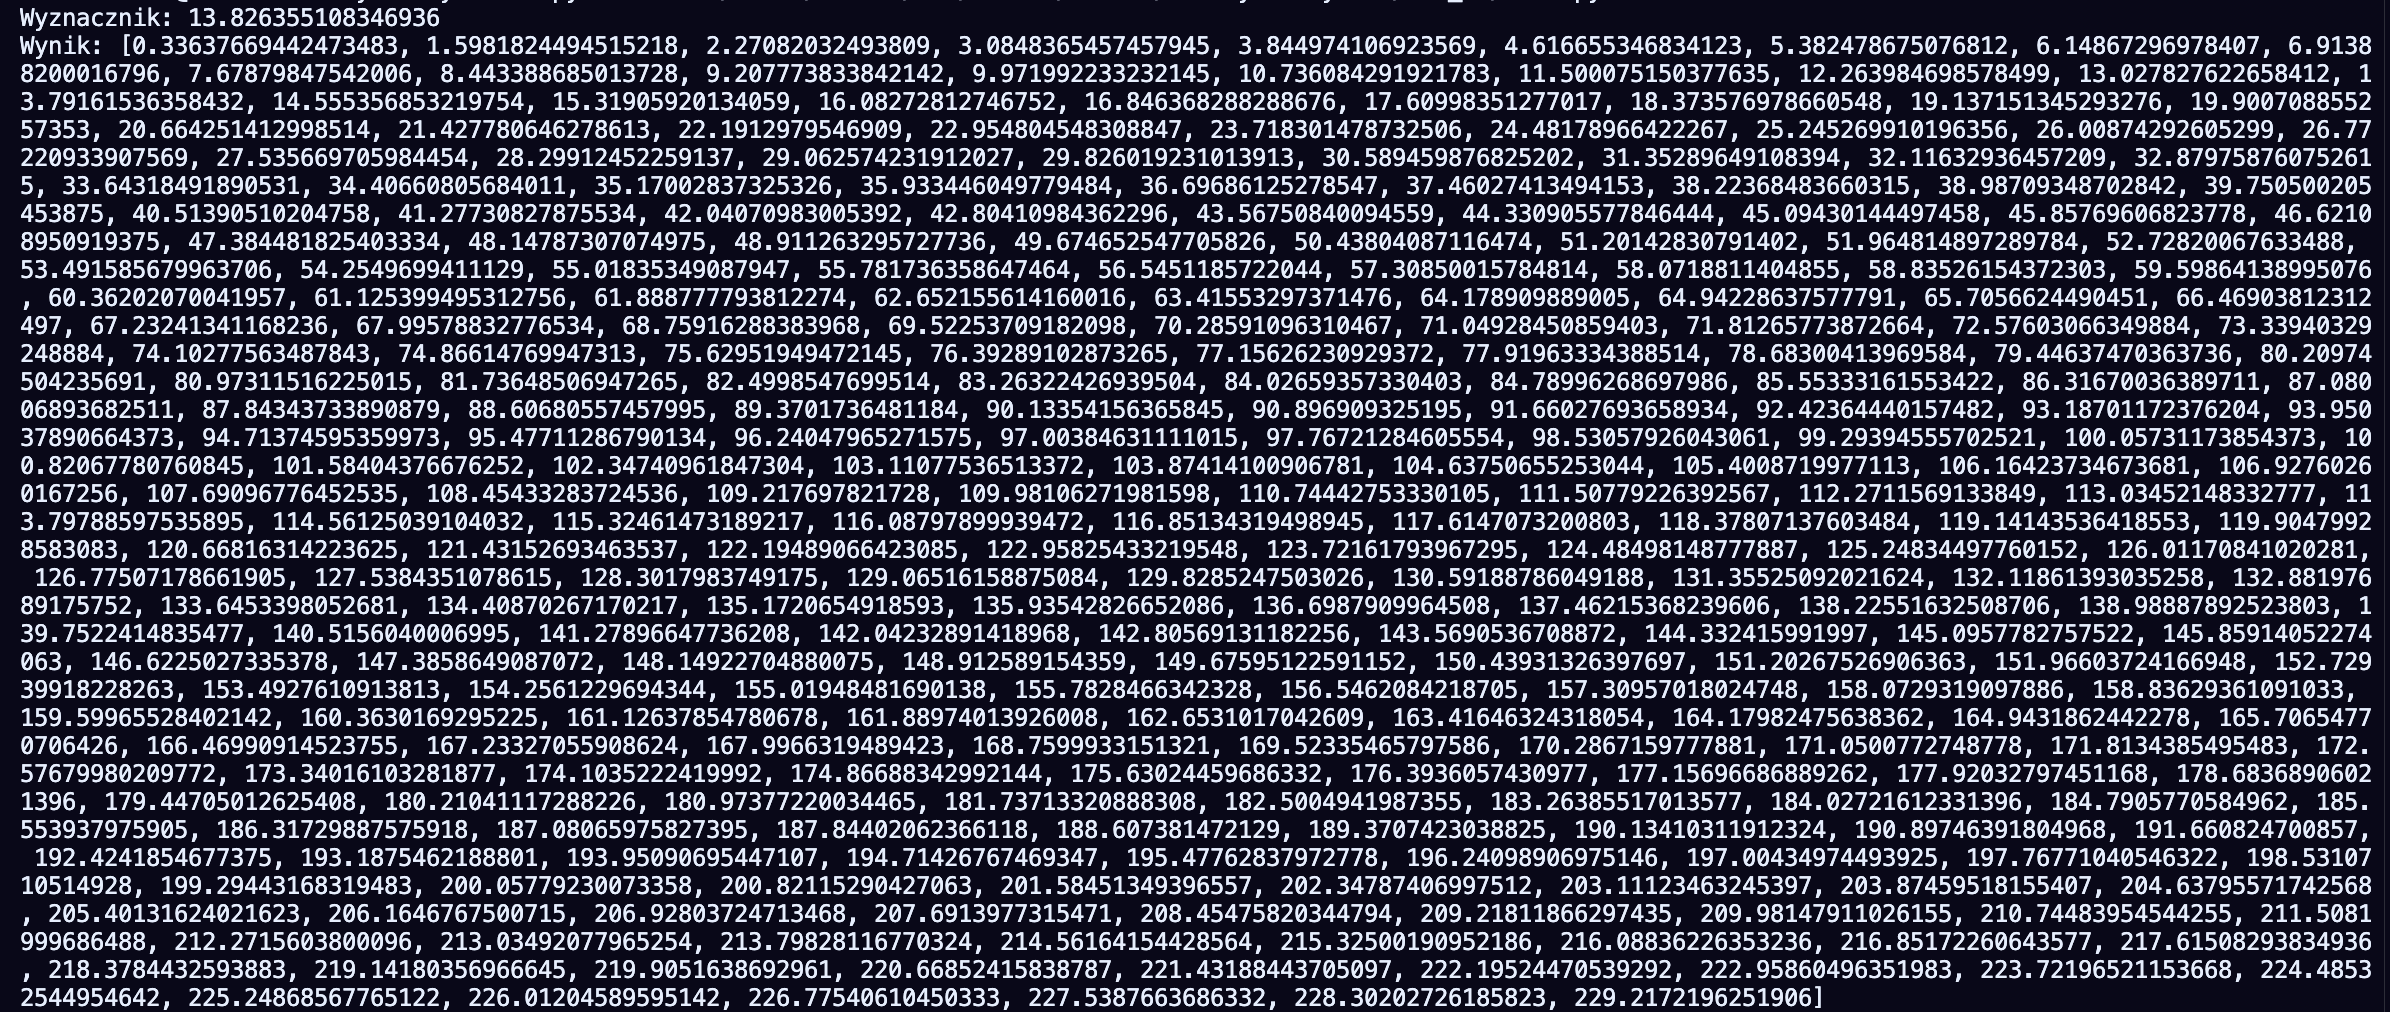
\includegraphics[width=0.8\textwidth]{output_screenshot.png}
    \caption{Zrzut ekranu przedstawiający wyniki programu.}
    \label{fig:output_screenshot}
\end{figure}

\subsection{Wykres czasowy}

Na poniższym wykresie przedstawiono zależność średniego czasu wykonania algorytmu od rozmiaru macierzy $N$. Aby uzyskać wiarygodne dane, dla każdej wartości $N$ program wykonywał algorytm \textbf{100 razy}, mierząc czas trwania każdego wykonania. Średnia arytmetyczna tych pomiarów została wykorzystana jako wartość reprezentatywna dla danego $N$. Dzięki temu wyeliminowano wpływ fluktuacji czasowych wynikających z obciążenia systemu czy innych czynników zewnętrznych.

\begin{figure}[h!]
    \centering
    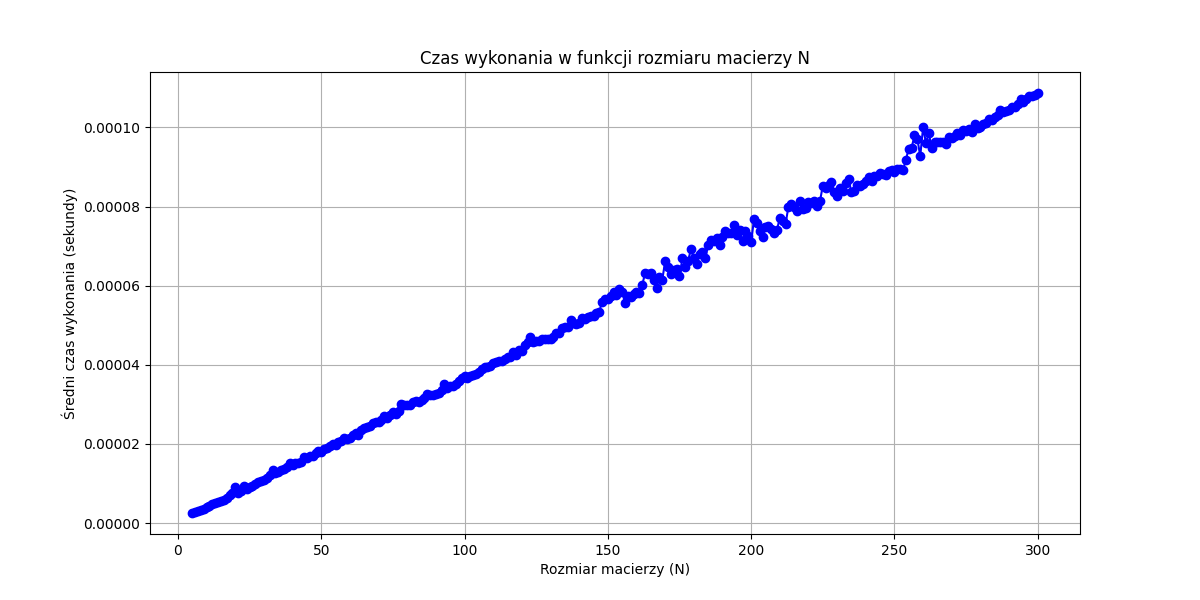
\includegraphics[width=0.8\textwidth]{execution_time_plot.png}
    \caption{Zależność czasu wykonania algorytmu od rozmiaru macierzy $N$.}
    \label{fig:execution_time_plot}
\end{figure}

\subsection{Wnioski z wyników}

Program poprawnie wyznacza wyznacznik macierzy czterodiagonalnej oraz rozwiązanie układu równań $y = A^{-1}x$. Uzyskane wyniki są zgodne z teoretycznymi oczekiwaniami:
\begin{itemize}
    \item Czas wykonania algorytmu rośnie liniowo wraz z rozmiarem macierzy $N$, co potwierdza teoretyczną złożoność obliczeniową $O(N)$.
    \item Wartość wyznacznika oraz rozwiązanie układu równań są stabilne i zgodne z założeniami algorytmu.
\end{itemize}


\section{Podsumowanie i wnioski}

Celem niniejszego zadania było wyznaczenie rozwiązania układu równań $y = A^{-1}x$, gdzie macierz $A$ była macierzą czterodiagonalną o specyficznej strukturze, oraz obliczenie wyznacznika tej macierzy. W ramach zadania opracowano i zaimplementowano algorytm wykorzystujący faktoryzację LU zoptymalizowaną dla macierzy czterodiagonalnych.

\subsection{Kluczowe wnioski}

\begin{itemize}
    \item Algorytm poprawnie uwzględnia strukturę macierzy czterodiagonalnej, przechowując jedynie cztery przekątne, co znacząco redukuje złożoność pamięciową i czasową.
    \item Rozwiązanie układu równań zostało wyznaczone efektywnie i zgodnie z oczekiwaniami dla wszystkich przetestowanych wartości $N$. Wektor $y$ wykazuje ciągłość i poprawność obliczeń.
    \item Wyznacznik macierzy $A$ został obliczony jako iloczyn elementów głównej przekątnej macierzy górnotrójkątnej $U$, co pozwoliło na szybkie i efektywne obliczenie tej wartości.
    \item Czas wykonania algorytmu rośnie liniowo wraz ze wzrostem rozmiaru macierzy $N$, co jest zgodne z teoretyczną złożonością obliczeniową $O(N)$. Przedstawiony wykres jednoznacznie potwierdza tę zależność.
\end{itemize}

\subsection{Wartość praktyczna rozwiązania}

Opracowany algorytm jest zoptymalizowany pod kątem macierzy o strukturze czteroprzekątnej. Rozwiązanie tego zadania ma szczególne znaczenie w kontekście rozwiązywania układów równań z macierzami rzadkimi, które pojawiają się m.in. w zagadnieniach numerycznych, modelowaniu fizycznym oraz analizie danych.

\subsection{Podsumowanie końcowe}

Zadanie zostało zrealizowane zgodnie z postawionymi wymaganiami. Opracowany program efektywnie rozwiązuje układ równań liniowych dla macierzy czterodiagonalnych oraz poprawnie oblicza wyznacznik macierzy. Algorytm został zoptymalizowany pod kątem wydajności i przeprowadzona analiza czasowa potwierdziła jego zgodność z teoretycznymi założeniami. Uzyskane wyniki są zgodne z oczekiwaniami i świadczą o poprawności zaimplementowanego rozwiązania.


\end{document}
